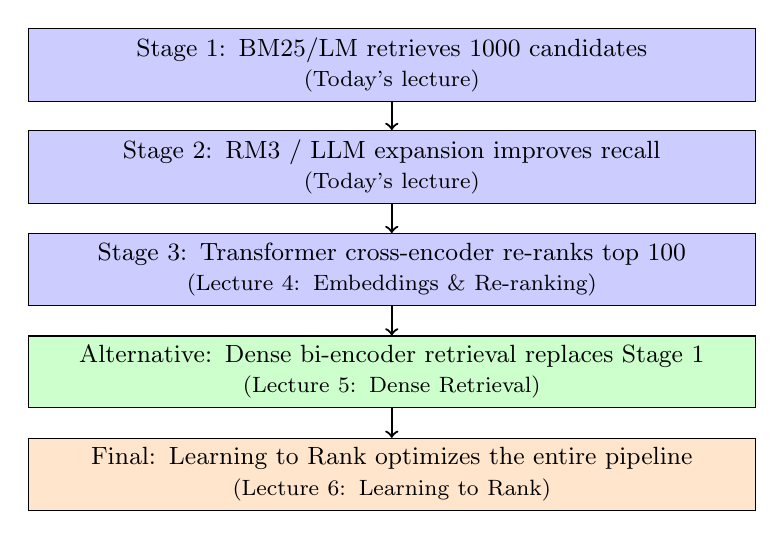
\begin{tikzpicture}[
    node distance=1.3cm,
    box/.style={rectangle, draw, fill=blue!20, text width=9cm, align=center, minimum height=0.9cm, font=\small},
    arrow/.style={->, thick}
]
    \node[box] (stage1) {Stage 1: BM25/LM retrieves 1000 candidates \\ \footnotesize (Today's lecture)};
    \node[box, below of=stage1] (stage2) {Stage 2: RM3 / LLM expansion improves recall \\ \footnotesize (Today's lecture)};
    \node[box, below of=stage2] (stage3) {Stage 3: Transformer cross-encoder re-ranks top 100 \\ \footnotesize (Lecture 4: Embeddings \& Re-ranking)};
    \node[box, below of=stage3, fill=green!20] (alt) {Alternative: Dense bi-encoder retrieval replaces Stage 1 \\ \footnotesize (Lecture 5: Dense Retrieval)};
    \node[box, below of=alt, fill=orange!20] (final) {Final: Learning to Rank optimizes the entire pipeline \\ \footnotesize (Lecture 6: Learning to Rank)};
    
    \draw[arrow] (stage1) -- (stage2);
    \draw[arrow] (stage2) -- (stage3);
    \draw[arrow] (stage3) -- (alt);
    \draw[arrow] (alt) -- (final);
\end{tikzpicture}
